\chapter{Reportes}
\label{mod:14-reportes}

\section{Propósito}
\label{sec:reportes-proposito}

Reportes \textbf{operativos de control} --- listados filtrables con totales, exportables a PDF/CSV, para auditar el día a día (qué se vendió, qué se compró, qué movió stock, qué movió caja). Es distinto de los reportes \textbf{analíticos} (KPIs agregados del dashboard), que son client-side con \code{jsPDF} y no forman parte de este módulo.

\section{Entidades principales}
\label{sec:reportes-entidades}

Este módulo no tiene entidades propias --- es una capa de agregación/exportación sobre entidades ya documentadas en el capítulo de Modelo de Datos (\S\ref{sec:modelo-datos}):

\begin{longtable}{p{4.6cm}p{9cm}}
\caption{Entidades fuente de cada reporte.}
\label{tab:reportes-entidades}\\
\toprule
\textbf{Reporte} & \textbf{Entidades fuente} \\
\midrule
\endfirsthead
\toprule
\textbf{Reporte} & \textbf{Entidades fuente} \\
\midrule
\endhead
\bottomrule
\endfoot
Ventas & \code{Venta}, \code{Cobro}, \code{VentaLinea} (Grupo C) \\
Compras & \code{PedidoProveedor}, \code{FacturaCompra}, \code{Recepcion}\allowbreak \code{Mercaderia} (Grupo C) \\
Movimientos de inventario & \code{MovimientoStock}, \code{vw_stock_actual} (Grupo B) \\
Movimientos de caja & \code{MovimientoCaja}, \code{SesionCaja} (Grupo C) \\
\end{longtable}

Dos campos se agregaron específicamente para este módulo (filtro de ``operador'' uniforme entre reportes): \code{Venta.VendedorId} ($\to$ \code{User}, quién creó la venta) y \code{Egreso.}\allowbreak \code{RegistradoPorId} ($\to$ \code{User}).

\section{Reglas de negocio clave}
\label{sec:reportes-reglas}

\begin{itemize}
  \item \textbf{Generación en backend, no client-side} --- decisión arquitectónica explícita por volumen (listados de miles de filas), consistencia de formato entre PDF y CSV, y para poder reutilizar el mismo exportador desde un futuro job de envío por email (los exportadores reciben el DTO, no el \code{HttpRequest}).
  \item \textbf{PDF con QuestPDF} (mismo patrón que \code{Movimiento}\allowbreak \code{Stock}\allowbreak \code{Pdf}\allowbreak \code{Generator} y la receta óptica), \textbf{CSV con un writer propio} (UTF-8 con BOM, separador \code{;}) --- sin librería nueva.
  \item \textbf{La matriz de filtros no es uniforme entre los 4 reportes}: fecha y sucursal son nativos en todos; en Inventario y Caja los demás filtros (categoría, método de pago) son nativos también, pero en Ventas y Compras ``método de pago'' y ``categoría'' son filtros de tipo ``contiene'' porque hay que atravesar \code{Cobro}/\code{VentaLinea} en vez de un campo directo.
  \item \textbf{Filtros combinables}: fechas, sucursal (scoping automático vía \code{ICurrent}\allowbreak \code{User}\allowbreak \code{Context}, igual que el resto del sistema --- ver \hyperref[adr:0009]{ADR 0009}), método de pago, categoría/producto, operador.
\end{itemize}

\section{Endpoints}
\label{sec:reportes-endpoints}

\begin{longtable}{p{1.3cm}p{6.4cm}p{6cm}}
\caption{Endpoints de Reportes.}
\label{tab:reportes-endpoints}\\
\toprule
\textbf{Método} & \textbf{Ruta} & \textbf{Descripción} \\
\midrule
\endfirsthead
\toprule
\textbf{Método} & \textbf{Ruta} & \textbf{Descripción} \\
\midrule
\endhead
\bottomrule
\endfoot
GET & \texttt{/api/reportes/ventas?}\allowbreak \texttt{desde\&hasta\&agrupacion} & Serie temporal agregada (día/semana/mes) \\
GET & \texttt{/api/reportes/citas?}\allowbreak \texttt{desde\&hasta\&agrupacion} & Turnos + consultas + recetas agregado \\
GET & \texttt{/api/reportes/inventario?}\allowbreak \texttt{desde\&hasta\&agrupacion} & Snapshot de stock (valorización, crítico, por categoría) + movimientos del rango \\
GET & \texttt{/api/reportes/compras?}\allowbreak \texttt{desde\&hasta\&agrupacion} & OC, facturas, recepciones, compras por proveedor \\
GET & \texttt{/api/reportes/}\allowbreak \texttt{operativo/\{tipo\}?}\allowbreak \texttt{desde\&hasta\&sucursalId\&}\allowbreak \texttt{metodoPago\&categoria\&}\allowbreak \texttt{operadorId\&tipoMov\&}\allowbreak \texttt{page\&pageSize} & Listado operativo paginado y filtrable (\code{tipo}: ventas\textbar compras\textbar inventario\textbar caja) \\
GET & \texttt{/api/reportes/}\allowbreak \texttt{operativo/\{tipo\}/}\allowbreak \texttt{export?formato\&...} & Archivo \code{application/pdf} o \code{text/csv}, mismos filtros sin paginar \\
\end{longtable}

\section{Flujo típico}
\label{sec:reportes-flujo}

\begin{figure}[htbp]
\centering
% Nombres de actor en dos lineas y node distance corto: con los nombres
% completos en una linea la figura mide ~25cm y no entra en los 16cm de
% ancho de texto.
\begin{tikzpicture}[node distance=1.1cm]
  \node[actor] (fe) {ReporteOperativo\\View};
  \node[actor, right=of fe] (api) {Reportes\\Controller};
  \node[actor, right=of api] (svc) {ReporteOperativo\\Service};
  \node[actor, right=of svc] (exp) {Reporte\\Exporter};

  \draw[lineavida] (fe.south) -- ++(0,-7);
  \draw[lineavida] (api.south) -- ++(0,-7);
  \draw[lineavida] (svc.south) -- ++(0,-7);
  \draw[lineavida] (exp.south) -- ++(0,-7);

  \draw[mensaje] ($(fe.south)+(0,-0.9)$) -- node[above,font=\scriptsize,align=center]{GET /reportes/\\operativo/ventas} ($(api.south)+(0,-0.9)$);
  \draw[mensaje] ($(api.south)+(0,-2.3)$) -- node[above,font=\scriptsize,align=center]{aplicar filtros +\\scoping por sucursal} ($(svc.south)+(0,-2.3)$);
  \draw[mensajeretorno] ($(svc.south)+(0,-3.5)$) -- node[below,font=\scriptsize]{página de resultados + totales} ($(fe.south)+(0,-3.5)$);
  \draw[mensaje] ($(fe.south)+(0,-4.8)$) -- node[above,font=\scriptsize,align=center]{GET .../export?formato\\(mismos filtros, sin paginar)} ($(api.south)+(0,-4.8)$);
  \draw[mensaje] ($(api.south)+(0,-6.0)$) -- node[above,font=\scriptsize,align=center]{traer TODAS\\las filas} ($(svc.south)+(0,-6.0)$);
  \draw[mensaje] ($(svc.south)+(0,-6.8)$) -- node[above,font=\scriptsize]{DTO completo} ($(exp.south)+(0,-6.8)$);
\end{tikzpicture}
\caption{Vista previa paginada vs.\ exportación completa: mismos filtros, dos caminos --- el export trae todas las filas sin paginar y las entrega como PDF (QuestPDF) o CSV (UTF-8+BOM).}
\label{fig:seq-reportes-export}
\end{figure}

\section{Vistas de frontend}
\label{sec:reportes-frontend}

\begin{itemize}
  \item \code{ReportesHubView.}\allowbreak \code{vue} --- landing con cards a cada reporte.
  \item \code{Reportes}\allowbreak \code{VentasView.}\allowbreak \code{vue}, \code{Reportes}\allowbreak \code{ComprasView.}\allowbreak \code{vue}, \code{Reportes}\allowbreak \code{InventarioView.}\allowbreak \code{vue}, \code{Reportes}\allowbreak \code{CitasView.}\allowbreak \code{vue} --- reportes analíticos (dashboard, no exportables por este módulo).
  \item \code{ReporteOperativoView.}\allowbreak \code{vue} --- vista \textbf{genérica} reutilizada para los 4 reportes operativos de este módulo (ventas/compras/inventario/caja), parametrizada por \code{tipo}.
\end{itemize}

\section{Interfaz}
\label{sec:reportes-interfaz}

\begin{figure}[htbp]
\centering
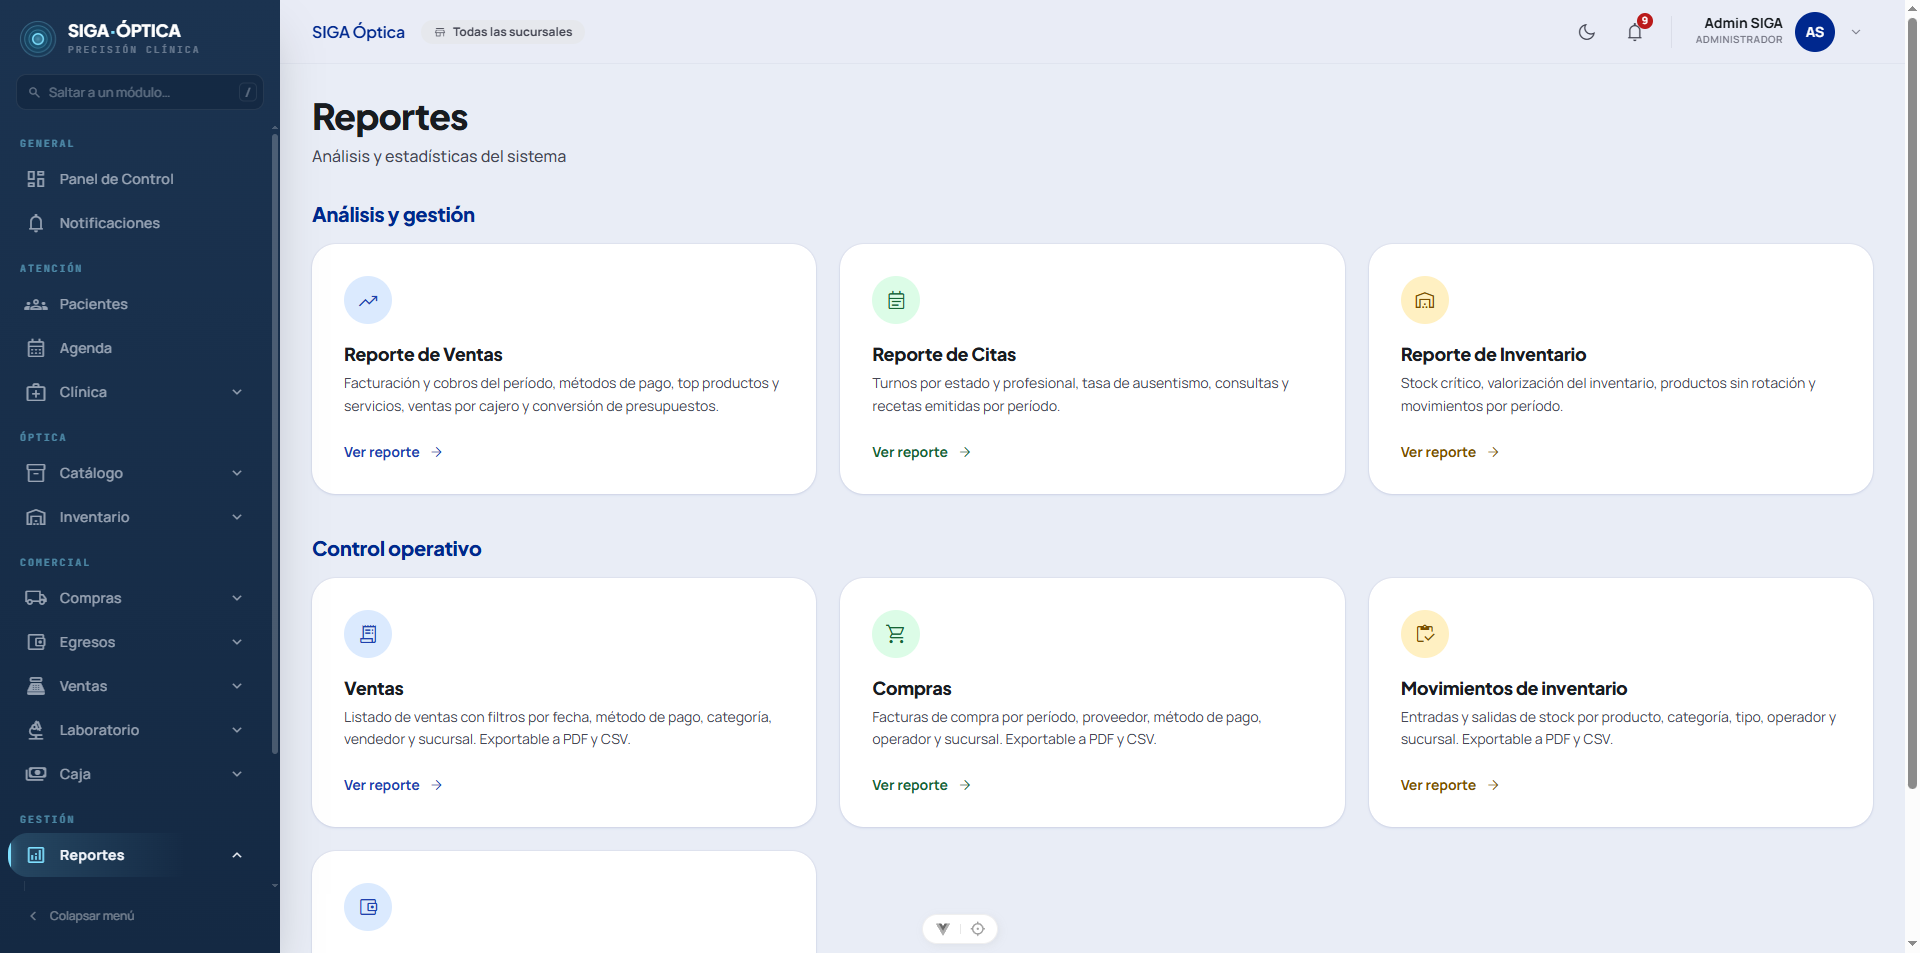
\includegraphics[width=0.95\textwidth]{imagenes/mod14-reportes.png}
\caption{Panel de acceso a los reportes gerenciales (ventas, citas, inventario) y operativos (ventas, compras, movimientos de inventario), exportables a PDF y CSV.}
\label{fig:mod14-reportes}
\end{figure}

\section{Estado}
\label{sec:reportes-estado}

\Implementado\ (backend \code{Reporte}\allowbreak \code{Operativo}\allowbreak \code{Service} + \code{ReporteExporter} + \code{Reportes}\allowbreak \code{Controller}; frontend \code{reportesOperativosService.}\allowbreak \code{ts} + \code{ReporteOperativoView.}\allowbreak \code{vue} + cards en \code{ReportesHubView}).
